\documentclass[12pt]{article}
\usepackage[a4paper, top=16mm, text={170mm, 248mm}, includehead, includefoot, hmarginratio=1:1, heightrounded]{geometry}
\usepackage{amsmath,amssymb,mathrsfs,amsthm,tikz,shuffle}
\usepackage{dsfont}


\theoremstyle{definition}
	\newtheorem{para}{}[section]
		\renewcommand{\thepara}{\thesection.\arabic{para}}
	\newtheorem{exa}[para]{Example}
\theoremstyle{plain}
	\newtheorem{lem}[para]{Lemma}
	\newtheorem{thm}[para]{Theorem}
	\newtheorem{pro}[para]{Proposition}
\renewcommand{\proofname}{Proof}


%+++++++++++++++++++++++数学字体的设置++++++++++++++++++++++++++++++++++++++++%
\newcommand{\me}{\mathrm{e}}  % for math e
\newcommand{\mi}{\mathrm{i}} % for math i
\newcommand{\dif}{\mathrm{d}} %for differential operator d
\newcommand{\cvec}[1]{\!\vec{\,#1}}
\newcommand{\Ptimes}{\,\overset{\otimes }{,}\,}
\DeclareSymbolFont{lettersA}{U}{txmia}{m}{it}
 \DeclareMathSymbol{\piup}{\mathord}{lettersA}{25}
 \DeclareMathSymbol{\muup}{\mathord}{lettersA}{22}
 \DeclareMathSymbol{\deltaup}{\mathord}{lettersA}{14}
 \newcommand{\uppi}{\piup}

\pagestyle{plain}

\begin{document}

\section{Intro}

\section{Map}

In this section we present a proof to the statement:
\begin{thm}
For an arbitrary product of M polynomials $P=\prod_{j=1}^M p_j^{\alpha_j}$, $p_j=\sum_{I_j} a_{I_j} x^{I_j}$ with $a_{I_j}\geq 0$ for all $I_j$ and
 \[
	x^{I_j}=\prod_{i=1}^N x_i^{n^{I_j}_i},
\]
whose Newton polytope is defined as the Minkowski sum  $N_P=\sum_j \alpha_j N(p_j)$, each $N(p_j)$ being the convex hull of vectors $\{\mathbf{n}^{I_j}=(n^{I_j}_1,\dots,n^{I_j}_N)\}$. Then the scattering map:
\[
	\mathbf X(x)=\frac{\partial \log P}{\partial \log \mathbf x},
\]
where $x_i\in (0,\infty)$ for all $i$, is a one-to-one map from $(0,\infty)^N$ to the interior of $N_P$ when matrix $(n_i^I)$ has full rank
\footnote{When matrix $(n_i^I)$ doesn't have full rank, the map is not one-to-one. But in fact, we can always assume it has full rank, thus $\dim (N(p))=N$. If not, there exists $\mathbf s\neq 0$ such that $\mathbf s \cdot \mathbf n^I=0$ for all $I$. In this case,
\[
	\mathbf s\cdot\mathbf X=\mathbf s\cdot\frac{\partial \log p}{\partial \log \mathbf x}=0.
\]
Therefore, one can project $\operatorname{im}(\mathbf X)$ by setting some $x_i=1$ so that there's no more vector $\mathbf s$ such that $\mathbf s\cdot \mathbf n^I=0$ for all $I$. Conversely, one can recover the original image by solving these equations $\mathbf s\cdot\mathbf X=0$}. 

\end{thm}

The proof is finished in two steps.:
\paragraph{Step 1: M=1}
Consider a unique polynomial $p=\sum_{I} a_I x^I$ with $a_I\geq 0$ for all $I$. The scattering map now reads:
\[
	\mathbf X(x)=\frac{\partial \log p}{\partial \log \mathbf x},
\]
where $x_i\in (0,\infty)$ for all $i$. Then the theorem is equivalent to the claim that the equations $\mathbf X(x)=\mathbf\Lambda$ have a solution in $\mathbb R^N$ iff $\mathbf\Lambda\in (N(p))^\circ$. Moreover, the solution is always unique for each interior point.


To prove the claim, let $\mathbf{\Lambda}$ be an interior point in $N(p)$ defined by 
\[
	\mathbf \Lambda=\sum_{I}\lambda_I\mathbf n^I
	=\frac{\partial}{\partial \log \mathbf x}\sum_{I}\lambda_I \log x^I
\]
where $\sum_I \lambda_I=1$ and $\lambda_I > 0$. Equations $\mathbf X(x)=\mathbf \Lambda$ are 
\[
\begin{aligned}
	0=\frac{\partial }{\partial \log \mathbf x}\left(
	\log p-\sum_{I}\lambda_I \log x^I
	\right)=\frac{\partial }{\partial \log \mathbf x}\left(
	\log F(\mathbf x)
	\right)=\frac{1}{F(\mathbf x)}\frac{\partial F(\mathbf x)}{\partial \log \mathbf x}
\end{aligned}
\]
where
\[
	F(\mathbf x)=\sum_I a_I x^I\prod_J (x^{-J})^{\lambda_J}.
\]
Let $\mathbf y=\log \mathbf x$, and then
\[
	\begin{aligned}
		F(\mathbf y)
		&=\sum_I a_I \exp\left(\mathbf{y}\cdot \left(\mathbf{n}^I-\mathbf{\Lambda}\right)\right)
	\end{aligned}
\]
so we only need to show that $F(\mathbf y)$ has a unique saddle points in $\mathbb R^N$ because $F>0$ for all $\mathbf y$.

 To see it, we firstly notice that $F(\mathbf y)$ is a strict convex function of $\mathbf y$. In fact, the Hessian of $F(\mathbf y)$ is 
\[
	H_{ij}(\mathbf y)=\frac{\partial^2}{\partial y_i\partial y_j}F(\mathbf y)=\sum_I a_I \exp\left(\mathbf{y}\cdot \left(\mathbf{n}^I-\mathbf{\Lambda}\right)\right)\left(\mathbf{n}^I-\mathbf{\Lambda}\right)_i\left(\mathbf{n}^I-\mathbf{\Lambda}\right)_j.
\]
For any $\mathbf v\neq 0$, 
\[
	\sum_{i,j}v_iv_jH_{ij}=\sum_I a_I \exp\left(\mathbf{y}\cdot \left(\mathbf{n}^I-\mathbf{\Lambda}\right)\right) \left(\mathbf v\cdot (\mathbf{n}^I-\mathbf{\Lambda})\right)^2 >0.
\]
It cannot vanish because that it only happens when $\mathbf v\cdot (\mathbf{n}^I-\mathbf{\Lambda})=0$ for all $I$. However, we have assumed $\{\mathbf n^I\}$ has full rank, {\it i.e. $dim(N(p))=N$}. Following the convexity of $N(p)$, vectors $\mathbf{n}^I-\mathbf{\Lambda}$ span the whole space $\mathbb R^N$. Thus a nonzero $\mathbf v$  making $\mathbf v\cdot (\mathbf{n}^I-\mathbf{\Lambda})=0$ for all $I$ cannot exist.

For a strict convex function $F(\mathbf y)$ on $\mathbb R^N$, it has a unique minimal in $\mathbb R^N$ iff it does not take its minimal when $\mathbf{y}$ goes to infinity along any direction. In our case, we only need that for any $\mathbf{y}\neq 0$ and $\mathbf\Lambda \in (N(p))^\circ $, there exist some $I$ such that  
\[
	\mathbf{y}\cdot (\mathbf{n}^I-\mathbf{\Lambda})>0,
\]
which is direct result from the convexity of $N(p)$: (figure \cite{}) If $\mathbf\Lambda \in (N(p))^\circ$, for a given $\mathbf y\neq 0$, the hyperplain $L$ with normal vector $\mathbf y$ crossing $\mathbf \Lambda$ divides the space $\mathbb R^N$ into semi-spaces $L^+$ and $L^-$, then $\mathbf{n}^I$ in $L^+$ are what we are looking for.

\begin{figure}[htbp]
\centering
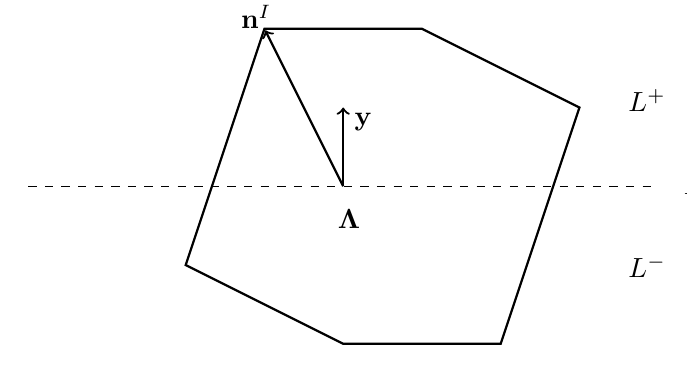
\begin{tikzpicture}
\draw[black,thick](3,0)--(1,0)--(0,-3)--(2,-4)--(4,-4)--(5,-1)--cycle;
\draw[black,dashed](-2,-2)--(6,-2);
\draw[->,black,thick](2,-2)--(2,-1);
\draw[->,black,thick](2,-2)--(1.01,-0.02);
\put(55,-72){$\mathbf{\Lambda}$};
\put(61,-35){$\mathbf{y}$};
\put(180,-60){$L$};
\put(160,-30){$L^+$};
\put(160,-90){$L^-$};
\put(20,0){$\mathbf{n}^I$};
\end{tikzpicture}


 

\end{figure}
Conversely, if $\mathbf\Lambda \not\in N(p)$, one can find a hyperplain $L$ such that $N(p)\subset L^-$, then the normal vector $\mathbf{y}$ of $L$ gives the wanted direction, making the exponentials all negative. $F(t\mathbf y)\to 0$ when $t\to \infty$. As a positive convex function, $F(\mathbf y)$ has no saddle point in $\mathbb R^N$.



Therefore, we have proven that $F(\mathbf y)$ has a unique minimal in $\mathbb R^N$ when $\mathbf \Lambda \in (N(p))^\circ$ and no saddle point in $\mathbb R^N$ when $\mathbf \Lambda \not\in N(p)$, which proves the claim. Hence, 
\[
	\mathbf X(x)=\frac{\partial \log p}{\partial \log \mathbf x},
\]
is an one-to-one map from $(0,\infty)^N$ to the interior of $N(p)$, which finishes the first step.



\paragraph{Step 2: general M}
Generally, let $\mathbf{\Lambda}$ be a interior point in Minkowski sum $\sum_p \alpha_p N(p)$ corresponding to $P=\prod_p p^{\alpha_p}$ defined by 
\[
	\mathbf{\Lambda}
	=\sum_p \alpha_p \mathbf{\Lambda}_p
	=\sum_p \alpha_p \sum_{I_p}\lambda_{I_p}\mathbf{n}^{I_p}
	=\frac{\partial}{\partial \log \mathbf{x}}\sum_{p}\alpha_p\sum_{I_p}\lambda_{I_p} \log x^{I_p}
\]
where $\sum_{I_p} \lambda_{I_p}=1$ and $\lambda_{I_p} > 0$. Equations $\mathbf{X}(x)=\mathbf{\Lambda}$ are 
\[
\begin{aligned}
	0=\frac{\partial }{\partial \log \mathbf{x}}\left(
	\log P-\sum_{p}\alpha_p\sum_{I_p}\lambda_{I_p} \log x^{I_p}
	\right)&=\frac{\partial }{\partial \log \mathbf{x}}\left(
	\log \left(\prod_p F_p^{\alpha_p}\right)
	\right),
\end{aligned}
\]
where
\[
	\begin{aligned}
		F_p(\mathbf y)&=\sum_{I_p} a_{I_p} \exp\left(\mathbf{y}\cdot \left(\mathbf{n}^{I_p}-\mathbf{\Lambda}_p\right)\right).
	\end{aligned}
\]
Write
\[
	F(\mathbf y)=\prod_p F_p(y)^{\alpha_p},
\]
we only need to show that $F(y)$ has a unique saddle point in $\mathbb R^N$.

We assume that $\alpha_p>0$ for all $p$. Here, $F(\mathbf y)$ is no longer a strict convex function. However, take a positive number $\alpha_0$ such that $\alpha_0< \alpha_p$ for all $p$, consider a new function
\[
	F(y)^{1/\alpha_0}=\prod_p F_p(y)^{\alpha_p/\alpha_0},
\]
since $F_p$ are convex functions and $\alpha_p/\alpha_0>1$, $F_p(y)^{\alpha_p/\alpha_0}$ are convex functions, so is their product. Since $F(y)^{1/\alpha_0}$ has the same minimums as $F(y)$, so we can further assume that $\alpha_p>1$ for all $p$.

Finally, we claim that $F(y)$ does not take minimum when $\mathbf{y}$ goes to infinity along any direction. It is because that for a given $\mathbf{y}$ and each $p$, $F_p(t\mathbf{y})\to \infty$ when $t\to \infty$, so does $F(t\mathbf{y})=\prod_p F_p(t\mathbf{y})^{\alpha_p}$. Therefore, equation $\mathbf{X}(x)=\mathbf{\Lambda}$ has a unique solution.

\section{Blow up}

Some review of positive geometry \& canonical form. blabla

Consider the integration
\begin{equation}\label{int}
	I(\alpha')=\int_{\mathcal P} \Omega_{\mathcal P}(x)\prod_i(p_i(x))^{\alpha' s_i},
\end{equation}
where $\Omega$ is the canonical form of the $D$-dimensional positive geometry $\mathcal P$, and we suppose $I(\alpha')$ is finite when $\alpha'>0$.
It's clear that $I(\alpha')$ diverge when $\alpha'\to 0$ because the simple pole of canonical form on the boundary of $\mathcal P$. We want to calculate the leading order of its Laurent series with respect to $\alpha'$ at $\alpha'=0$. % It's a rational function of $s_i$ since $p_i$ are all polynomials.

% Consider the following integral
% \[
% 	\int_{\mathbb R_+^d}\frac{d x_1}{x_1} \cdots \frac{d x_d}{x_d} x_1^{n_1}\cdots x_d^{\alpha' n_d} P(x_1,\dots,x_d)^{-\alpha' c}, 
% \]
% where $P$ is a polynomial, here we can further assume that $P(0,\dots,0)\neq 0$. When $\alpha'\to 0$, the integral diverge, we want to calculate the leading term of $(\alpha')^{-1}$ of this integral. blabla

Let's first consider the one-dimensional example, the Beta function 
\[
	B(\alpha' a,\alpha' b)=\int_0^1 \frac{dt}{t(1-t)}\, t^{\alpha' a}(1-t)^{\alpha' b}.
\]
To calculate the integral, we can decompose the integral by 
\[
	\biggl(\int_{0}^\epsilon +\int_\epsilon^{1-\epsilon}+\int_{1-\epsilon}^1\biggr) \frac{dt}{t(1-t)}\, t^{\alpha' a}(1-t)^{\alpha' b}.
\]
The middle integral is finite when $\alpha'\to 0$ so that it does not contribute, the other two integrals are
	\[
		\int_0^\epsilon  \frac{dt}{t(1-t)}\, t^{\alpha' a}(1-t)^{\alpha' b}
	\sim \int_0^\epsilon \frac{dt}t t^{\alpha' a} 
	= \frac{\epsilon^{\alpha' a}}{\alpha'a} \sim \frac{1}{\alpha'a},
	\]
\[
	\int_{1-\epsilon}^1  \frac{dt}{t(1-t)}\, t^{\alpha' a}(1-t)^{\alpha' b}
	\sim \int_0^\epsilon \frac{dt}{t}\, t^{\alpha' b} \sim \frac{1}{\alpha' b},
\]
so the leading term of this integral is 
\[
	B(\alpha' a,\alpha' b)\sim\frac 1{\alpha'}\biggl(\frac 1a+\frac 1b\biggr).
\]

One important lesson from the above trivial integral is that the leading terms of the integral come from the vertices of the positive geometry. 

Now let's come to the two-dimensional example,
\[
	I=\int_{\mathbb R_1+^2} \frac{dx}{x}\frac{dy}{y}x^{\alpha' a}y^{\alpha' b}(x+y)^{-\alpha' c}.
\]
The leading terms come form the neighbourhoods of four vertices $(0,0)$, $(0,\infty)$, $(\infty,0)$ and $(\infty,\infty)$. Let's consider the simplest vertex first, 
\[
	I(0,\infty)=\int_{0}^\epsilon\int_{1/\epsilon}^\infty \frac{dx}{x}\frac{dy}{y}x^{\alpha' a}y^{\alpha' b}(x+y)^{-\alpha' c}\sim \int_{0}^\epsilon\int_{1/\epsilon}^\infty \frac{dx}{x}\frac{dy}{y}x^{\alpha' a}y^{\alpha' (b-c)}\sim 
	\frac{1}{{\alpha'}^2}\frac{1}{a} \frac{1}{c-b}
\]
similarly, $I(\infty,0)\sim ({\alpha'}^2 b (c-a))^{-1}$. Near the vertex $(0,\infty)$, the integral decouples because the mixed factor $x+y \sim y$ when $y \gg x$.  

Now consider the harder vertex
\[
	I(0,0)=\int_{0}^\epsilon\int_0^{\epsilon} \frac{dx}{x}\frac{dy}{y}x^{\alpha' a}y^{\alpha' b}(x+y)^{-\alpha' c}.
\]
When $(x,y)\to (0,0)$, we cannot decouple $x$ and $y$ in the mixed factor $(x+y)^{-\alpha' c}$ because we don't know which one is dominated. A clever way to calculate it is blowing-up. Let $x = tp$ and $y=t(1-p)$, then
\begin{equation}\label{canonicalformunderblowup}
	\frac{dxdy}{xy} = \frac{dp}{p(1-p)}\frac{dt}{t},
\end{equation}
and
\begin{equation*}
	I(0,0)=\int_{0}^\epsilon\frac{dt}{t} t^{\alpha'(a+b-c)}\int_0^{1}\frac{dp}{p(1-p)}p^{\alpha' a}(1-p)^{\alpha' b}%\sim \frac{1}{\alpha'}\frac{1}{a+b-c}\int_0^{1}\frac{dp}{p(1-p)}p^{\alpha' a}(1-p)^{\alpha' b}
	\sim \frac{1}{{\alpha'}^2}\frac{1}{a+b-c}\biggl(\frac 1a+\frac 1b\biggr).
\end{equation*}
In this example, whether $x$ or $y$ is dominated in the integration is characterized by $p$, and both vertices $p\sim 0$ ($x\ll y$) and $p\sim 1$ ($y\ll x$) contribute. Similarly, 
\[
	I(\infty,\infty)\sim \frac{1}{{\alpha'}^2}\frac{1}{c-a-b}\biggl(\frac 1{c-a}+\frac 1{c-b}\biggr),
\]
so the leading terms of original integral is 
\[
	I\sim I(0,0)+I(0,\infty)+I(\infty,0)+I(\infty,\infty).
\]

Now let's consider the general story. Generally, the integral near a vertex need not to be decoupled as $I(0,\infty)$ above, so blowing-up is necessary. Suppose we come to the vertex defined locally by $x_1=\cdots=x_D=0$, 
\[
	I(0,\dots,0)\sim \int_{[0,\epsilon]^D} \frac{d x_1}{x_1}\cdots \frac{d x_D}{x_D} \prod_i(p_i(x))^{\alpha' s_i}.
\]
In each polynomial $p_i$, 
\[
	p_i(x)=\sum_{I} a_{iI} x^{n^I},
\]
we need to worry about which $x^{n^I}$ is dominated in the integration, however not all terms can  dominate the integral. For example, if we find that $x^{n^J}=x^{n^I}x^{v}$ or equivalently $n^J=n^I+v$ for some non-zero positive vector $v$, there's no need to consider $x^{n^J}$ anymore because it goes to zero faster than $x^{n^I}$. 

More formally, for a polynomial $p(x)=\sum_{I\in \mathscr A}a_I x^{n^I}$ we can choose a basis of $\{n^I\}_{I\in \mathscr B}$ such that for all $I \in \mathscr A-\mathscr B$, there exist non-negative numbers $\{c^I_J\}$ such that
\[
	n^I = \sum_{J\in \mathscr B}c^I_J n^J,\quad \sum_J c^I_J>  1,
\]
and then we can replace $p(x)$ by a new polynomial $\bar p(x)=\sum_{J\in \mathscr B}a_J x^{n^J}$ because for all $I \in \mathscr A-\mathscr B$ it goes to zero faster than at least one $x^{n^J}$. In fact, after setting $x_i=t y_i$, for $I \in \mathscr A-\mathscr B$, 
\[
	x^{n^I}=\prod_J (x^{n^J})^{c^I_J}=x^{\sum_J c^I_J n^J} = t^{\sum_J c^I_J |n^J|}y^{\sum_J c^I_J n^J}
\]
where there always exists a $K\in \mathscr B$ such that $|n^K|<\sum_J c^I_J |n^J|$, otherwise
\[
	\sum_{K\in \mathscr B} c^I_K|n^K|\geq \left(\sum_{K\in \mathscr B} c^I_K\right)\sum_{J\in \mathscr B} c^I_J |n^J|>\sum_{J\in \mathscr B} c^I_J |n^J|,
\]
so there's a contradiction.

Geometrically, if we consider the cone $C$ spanned by all $\{n^I\}$, then the basis can be choosen as the vertices on the boundary of $C$, and terms corresponding to points inside $C$ can be dropped.
For example, suppose that $p(x,y)=x^3+y^3+xy+x^3y^2+xy^3$, we draw each $n^I$ in the following diagram,
\begin{center}
	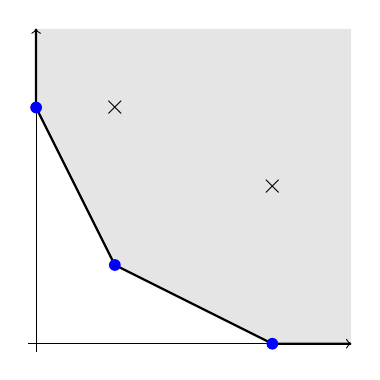
\begin{tikzpicture}
		\fill[gray!20] (0,4) -- (0,3) -- (1,1) -- (3,0) -- (4,0) -- (4,4);
		\draw[thick] (0,4) -- (0,3) -- (1,1) -- (3,0) -- (4,0);
		\draw[->](-0.1,0) -- (4,0);
		\draw[->](0,-0.1) -- (0,4);
		\node at (3,2) {$\times$};
		\node at (1,3) {$\times$};
		\node[inner sep=1.5pt,circle,fill=blue] at (0,3) {};
		\node[inner sep=1.5pt,circle,fill=blue] at (1,1) {};
		\node[inner sep=1.5pt,circle,fill=blue] at (3,0) {};
	\end{tikzpicture}
\end{center}
where $x^3y^2\leftrightarrow (3,2)$ and $xy^3\leftrightarrow (1,3)$ are represented by $\times$ in the diagram and other terms are represented by blue points. The basis is given by blue points $\{x^3\leftrightarrow (3,0),y^3\leftrightarrow (0,3),xy\leftrightarrow (1,1)\}$, and the gray region is the set of all vectors $v=\sum_{J\in \mathscr B}c^I_J n^J$ where $\sum_J c^I_J>1$, therefore we throw away terms in the gray region and then get that $\bar p(x)=x^3+y^3+xy$. 

Now we start to consider how to blow up. As has seen from eq.\eqref{canonicalformunderblowup}, one important feature of $\Omega_{\mathcal P}$ is `invariant' under the blowing-up because the residue of the canonical form on the boundary is the canonical form of the boundary.

Suppose we blow up near the boundary defined locally by $x_1=\cdots=x_n=0$ in integral eq.\eqref{int}. Now let $x_i=ty_i$, where $[y_1,\dots,y_n]$ are positive projective coordinates. Near the boundary, the canonical form of $\Omega$ performs as 
\[
	\Omega=\frac{dx_1}{x_1}\wedge \cdots\wedge\frac{dx_n}{x_n}
	\wedge \Phi(x')+O(t^0),
\]
where $x'$ are other coordinates. In new coordinates, it can be written as 
\[
	\Omega=\frac{1}{y_n}\frac{dt}{t}\wedge \frac{dy_1}{y_1}\wedge \cdots\wedge\frac{dy_{n-1}}{y_{n-1}}\wedge \Phi(x')+O(t^0),
\]
where $y_n=1-(y_1+\cdots+y_{n-1})$ and $\Phi$ is the canonical form of the boundary of $\mathcal P$ given by $x_1=\cdots=x_n=0$. Therefore,
\[
	\operatorname{Res}_{t=0}(\Omega)=\frac{1}{y_n}\frac{dy_1}{y_1}\wedge \cdots\wedge\frac{dy_{n-1}}{y_{n-1}}\wedge \Phi(x')=\Omega_{n-1}(y)\wedge \Phi(x'),
\]
$\Omega_{n-1}(y)$ the canonical form of a standard $(n-1)$-dimensional simplex $\Delta_{n-1}$. 
% If we rewrite it in new coordinates $\{z_i\}$ such that
% \[
% 	z_0=0,\quad y_i=z_i-z_{i-1},\quad z_{n}=1,
% \]
% then 
% \[
% 	\Omega_{n-1}(z)=\frac{dz_1\wedge\cdots\wedge dz_n}{(z_1-z_0)\cdots (z_n-z_{n-1})}.
% \]
% It's the more familiar form.

% Consider a set of irreducible polynomials $\{p_i\}$, let $Z(p_i)$ be the zero point set of $p_i$ in $\mathbb{R}^n$. Suppose a curved polytope $\mathcal P$ is bounded by $\bigcup_i Z(p_i)$, if $F_k$ is a codimension $k$ face of $\mathcal P$ where $\#\{i\,:\,F_k\subset Z(p_i)\}>k$, then we call it a degenerated face.

% Now Consider the integration
% \[
% 	I(\alpha')=\int_{\mathcal P} \Omega_{\mathcal P}(x)\prod_i(p_i(x))^{\alpha' s_i},
% \]
% where $\Omega$ is the canonical form of $\mathcal P$, and we suppose $I(\alpha')$ is finite when $\alpha'>0$.
% It's clear that $I(\alpha')$ diverge when $\alpha'\to 0$. We want to find all possible poles in the leading order of its Laurent series with respect to $\alpha$ at $\alpha=0$. It's a rational function of $s_i$ since $p_i$ are all polynomials.

% If $F$ is a facet of $\mathcal P$. Locally, if $F$ is defined by $x=0$, then near $F$, the integration is 
% \[
% 	\int_0^\epsilon \frac{d x}{x} x^{\alpha' a} \int_{x'}\Psi(x')
% 	\sim \frac{1}{\alpha' a}\int_{x'}\Psi(x'),
% \]
% where $x'$ are other coordinates and $\Psi(x')$ is the left part of $\Omega_{\mathcal P}(x)\prod_i(p_i(x))^{\alpha' s_i}$.

What's more, suppose polynomials are factorized into
\[
	p_i(x) = t^{k_i}q_i(x',y,t).
\]
Therefore, the integral, near this boundary and when $\alpha'$ is small, becomes
\[
	\begin{aligned}
		\int_{x'} \int_{x\in [0,\epsilon]^n} \Omega(x,x')\, \prod_i(p_i(x))^{\alpha' s_i}
		&=
		\int_0^\epsilon \, \frac{dt}{t} t^{\alpha' \sum_i k_is_i}\int_{y\in\Delta_{n-1}}\int_{x'}\Omega_{n-1}(y)
		\Phi(x')\prod_i
		(q_i(x',y,t))^{\alpha' s_i},
	\end{aligned}
\]
however we still need to worry about the blowing-up of $t$, $y$ and $x'$.

\section{Application and Example}

% string Z integral, Cn, Gkn ...

\end{document}